\section{Sieve diagrams}\label{sec:twoway-sieve}
\ixon{sieve diagram}
\epigraph{They consider me to have sharp and penetrating vision because I see
them through the mesh of a sieve.}{Kahlil Gibran}
For two- (and higher-) way \ctabs{}, the
design principles of perception, detection, and comparison
(see \chref{ch:intro})
suggest that we should try to show the observed frequencies
in relation to what we would expect those frequencies to be
under a reasonable null model---for example, the
hypothesis that the row and column variables are unassociated.

To this end, several schemes for representing \ctabs\
graphically are
based on the fact that when the row and column variables are
independent, the estimated expected frequencies, \(m_{ij}\), are
products of the row and column totals (divided by the grand total).
\begin{equation*}
 m_{ij} = \frac{ n_{i+} n_{+j} } { n_{++} }
 \period
\end{equation*}
Then, each cell can be represented by a rectangle whose area shows
the cell frequency, \(n_{ij}\),  or deviation from independence.

For example, for any two-way table, the expected frequencies under independence
can be represented by rectangles whose widths are proportional to the
total frequency in each column, \(n_{+j}\), and whose heights are
proportional to the total frequency in each row, \(n_{i+}\); the area
of each rectangle is then proportional to \(m_{ij}\). \figref{fig:sieve0}
shows the expected frequencies for the hair and eye color
data (\tabref{tab:hairdat}).

This display simply represents the model---what the frequencies would
be if hair color and eye color were independent---not the data.
Note, however, that the rectangles are cross-ruled so that the number of
boxes in each (counting up the fractional bits) equals the expected
frequency with which the cell is labeled, and moreover, the
rulings are equally spaced in all cells.
Hence, cross-ruling the cells to show the observed frequency
would give a data display which implicitly compares observed
and expected frequencies.

\begin{figure}[htb]
  \centering
  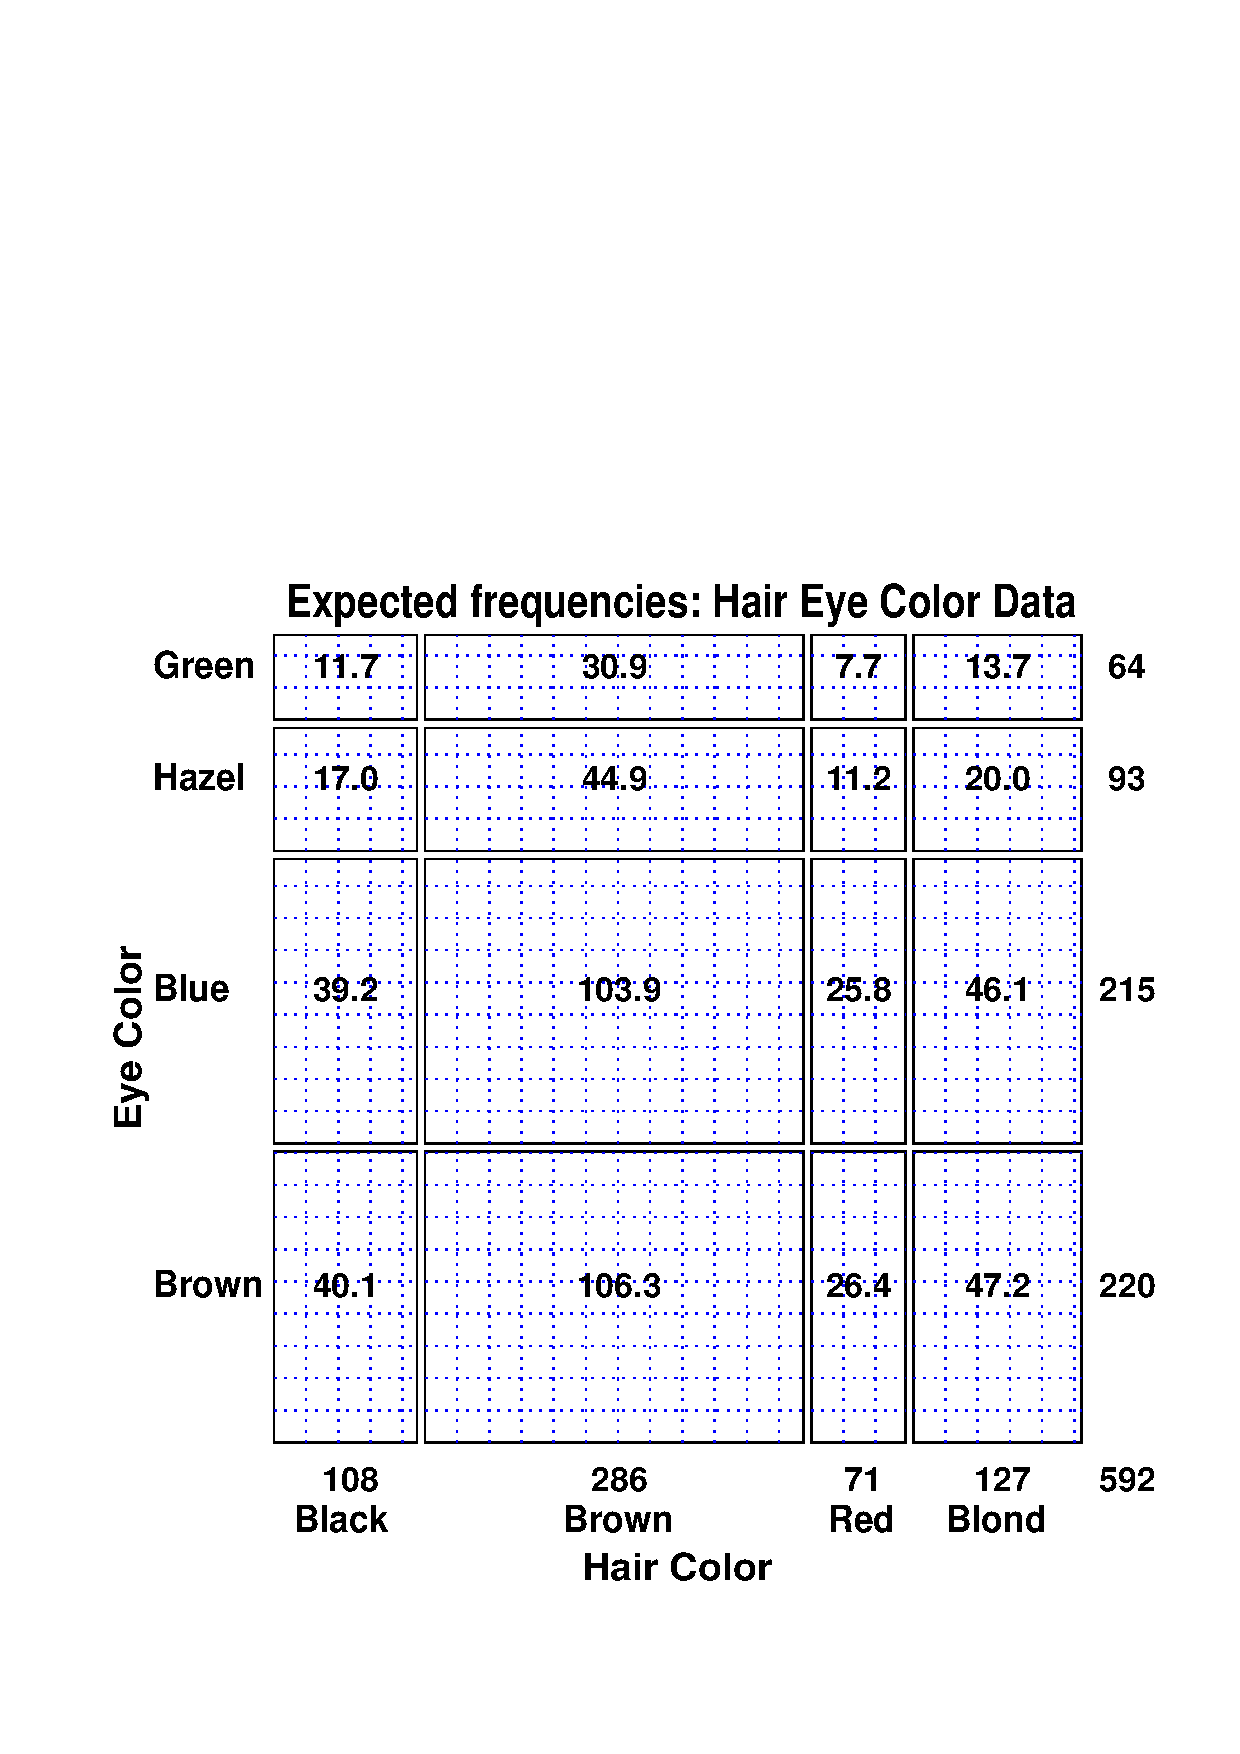
\includegraphics[scale=.5]{ch3/fig/sieve0}
  \caption[Expected frequencies under independence]{Expected frequencies under independence.  Each box has area equal to its expected frequency, and is cross-ruled proportionally to the expected frequency.}\label{fig:sieve0}
\end{figure}


Riedwyl and Sch\"{u}pbach
\citeyear{RiedwylSchupbach:83,RiedwylSchupbach:94}
%(1983, 1994)
proposed a
\glossterm{sieve diagram}
(later called a \glossterm{parquet diagram}) based on
this principle.  In this display the area of each rectangle is
proportional to expected frequency,
as in \figref{fig:sieve0},  but observed frequency is shown by
the number of squares in each rectangle.  Hence, the difference
between observed and expected frequency appears as variations in the density of
shading.
Cells whose observed frequency $n_{ij}$ exceeds the expected $m_{ij}$
appear denser than average.
The pattern of positive and negative deviations from independence
can be more easily seen by
using color, say, red for negative deviations, and blue for positive.%
\footnote{
Positive residuals are also shown by solid lines, negative residuals by broken
lines, so that they may still be distinguished in monochrome versions.}

\begin{Example}[haireye2]{Hair color and eye color}
The sieve diagram for hair color and eye color (\tabref{tab:hairdat})
is shown in
\figref{fig:sieve1}.
The pattern of color and shading shows the high frequency of
blue-eyed blonds and people with brown eyes and dark hair.
People with hazel eyes are also more likely to have red or brown hair,
and those with green eyes more likely to have red or blond hair,
than would be observed under independence.

\begin{figure}[htb]
  \centering
  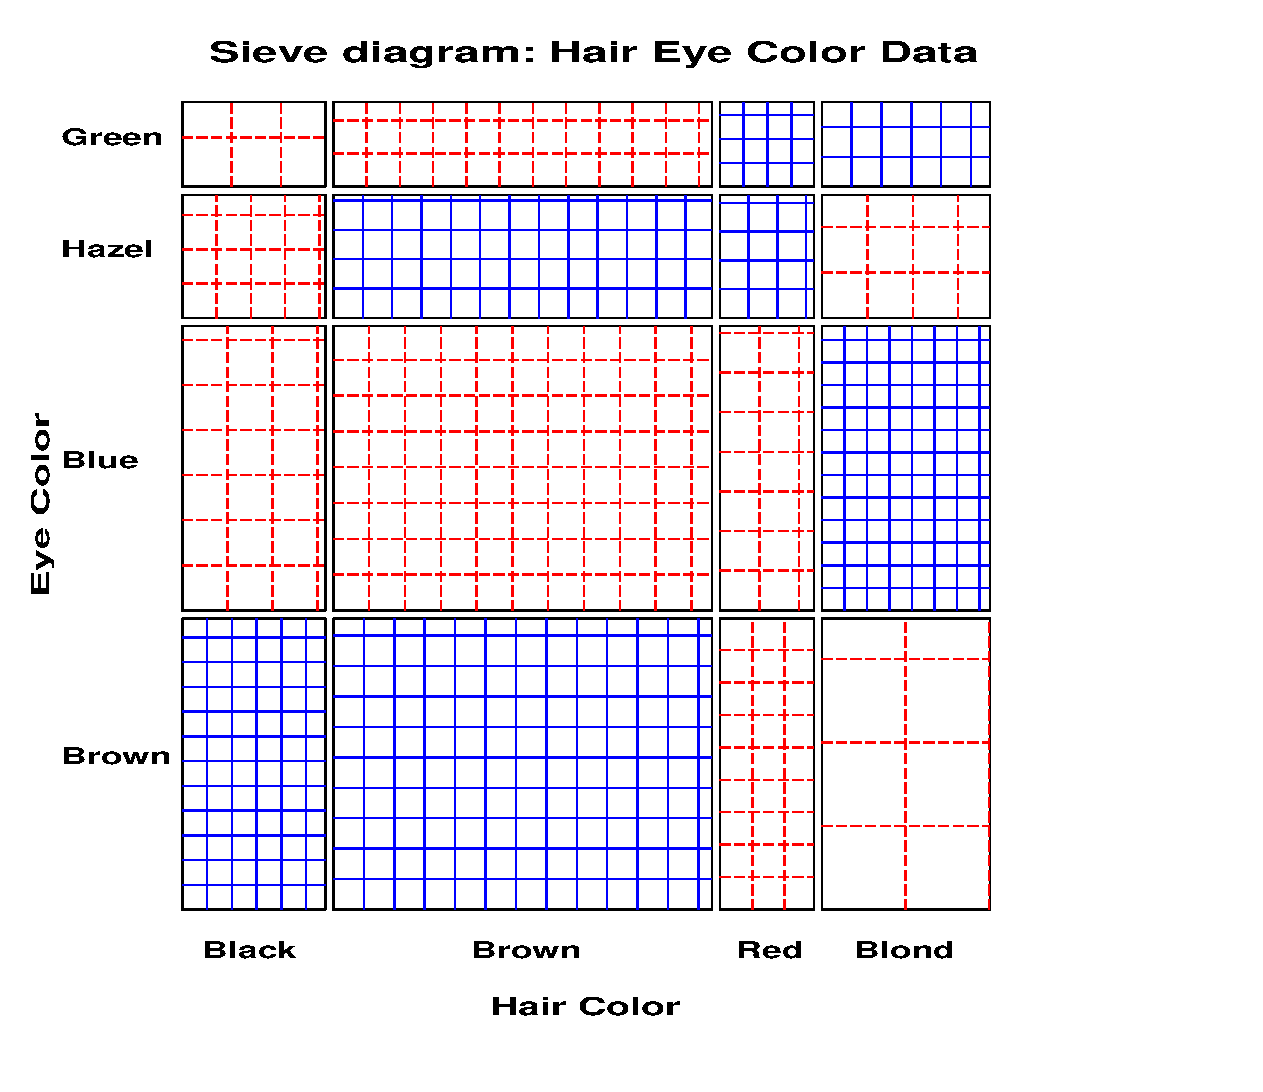
\includegraphics[scale=.5]{ch3/fig/sieve1}
  \caption[Sieve diagram for hair-color, eye-color data]{Sieve diagram for hair-color, eye-color data.  Observed frequencies are equal to the number
  squares in each cell, so departure from independence appears as variations
  in shading density.}\label{fig:sieve1}
\end{figure}
\ixd{hair-eye color}
\end{Example}

\begin{Example}[vision1]{Visual acuity}
\figref{fig:sieve2} shows the sieve diagram for data on visual acuity in a large
sample of women ($n=7477$) aged 30-39, working in the U.K.
Royal Ordnance factories during World War II
(\citet[Table 33.5]{KendallStuart:61},
\citet[p. 284]{Bishop-etal:75}).
For each person, unaided distance vision of each eye was measured
and categorized into four ordered grades.  The data are listed in
\datref{dat:vision}.

The diagonal cells show the obvious:
people tend to have the same visual acuity in both eyes, and there is
strong lack of independence.  The off diagonal cells show a more subtle
pattern which suggests symmetry---the cells below the diagonal
are approximately equally dense as the corresponding cells above the diagonal.
Moreover, the relatively consistent pattern on the diagonals
$\pm 1, \pm 2, \dots$ away from the main diagonals suggests
that the association may be explained in terms of the \emph{difference}
in visual acuity between the two eyes.
These suggestions can be tested by fitting  intermediate models
between the null model of independence (which fits terribly)
and the saturated model (which fits perfectly),
as we shall see later in this book.
A model of quasi-independence, for example (\exref{ex:victims})
ignores the diagonal cells and tests whether independence holds
for the remainder of the table.
%\aunote{Xref?}
\ixd{visual acuity}

\begin{figure}[htb]
  \centering
  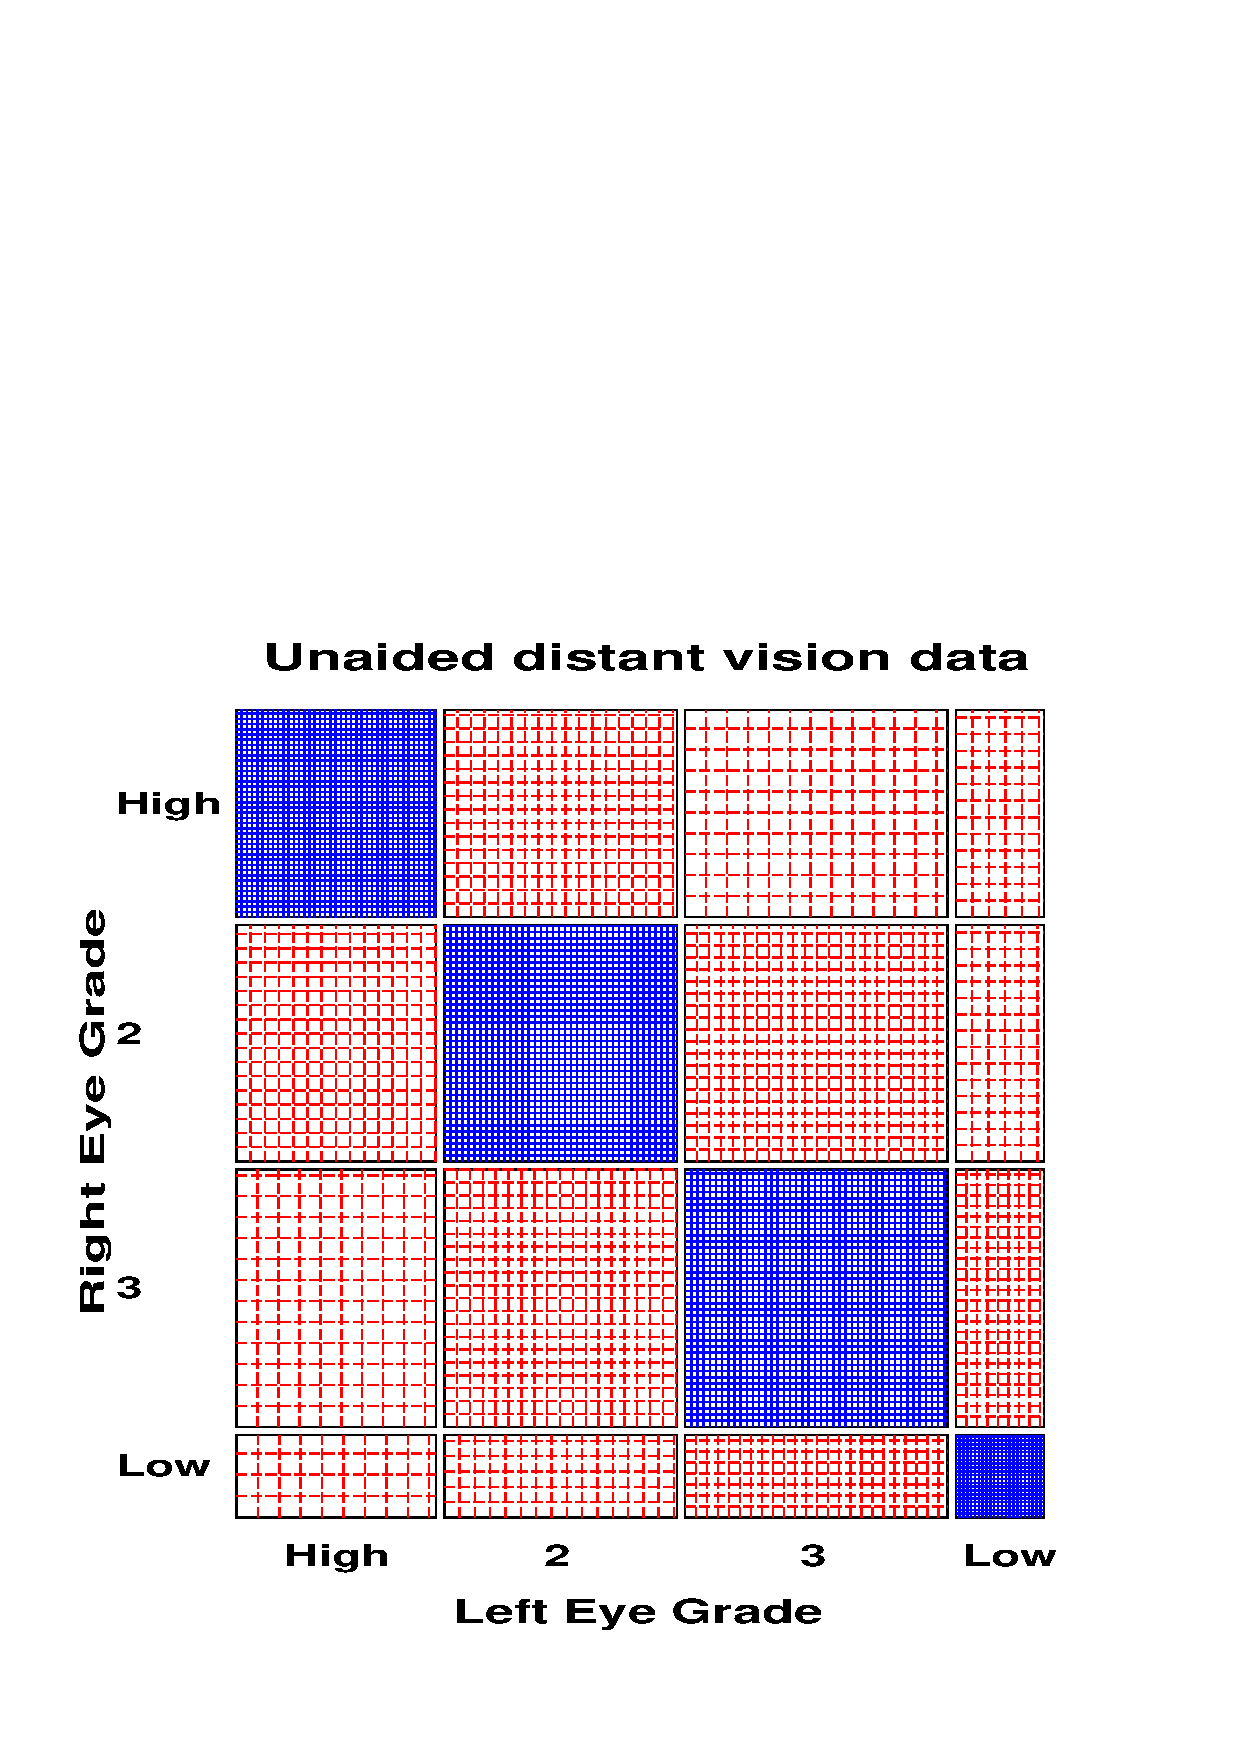
\includegraphics[scale=.5]{ch3/fig/sieve2}
  \caption{Vision classification data for 7477 women}\label{fig:sieve2}
\end{figure}
\end{Example}

\subsection{The \sasprog{SIEVE}}
Sieve diagrams are implemented as a general module in \IML{},
because the calculations and graphics are most easily handled using
matrices.
The program is listed and documented in \macref{mac:sieve}.

To use the program, \texttt{\%include} the \sasprog{SIEVE}
within a \PROC{IML} step.  Then
enter the observed frequencies in an array \texttt{f},
and create a character vector \texttt{vnames} containing
the row and column variable names, and a two-row
character matrix \texttt{lnames} containing the
category labels.
The sieve diagram is produced with the \texttt{sieve} module,
\begin{listing}
run sieve( f, vnames, lnames, title );
\end{listing}
For example, the sieve diagram in \figref{fig:sieve1}
for the hair color eye color data is produced by the
statements below.
Note that the graphics options \texttt{hsize} and \texttt{vsize}
should be set to make the plot square.
%% input: /users/faculty/friendly/sasuser/catdata/sievehair.sas
%% last modified: 05-Jan-98  9:15
\begin{listing}
goptions hsize=7in vsize=7in;
 
filename sieve '~/sasuser/catdata/sieve.sas';
proc iml;
   %include sieve;
   f = \{   5   29  14  16 ,       /* green */
          15   54  14  10 ,       /* hazel */
          20   84  17  94 ,       /* blue  */
          68  119  26   7 \};      /* brown */
 
   vnames = \{'Eye Color' 'Hair Color'\};
   lnames = \{'Green' 'Hazel' 'Blue' 'Brown' ,
             'Black' 'Brown' 'Red'  'Blond'\};
   title  = 'Sieve diagram: Hair Eye Color Data';
   font='hwpsl011';
   run sieve(f, vnames, lnames, title );
quit;
\end{listing}


\subsection{Larger tables}
\ix{interactive coding}
\ix{sieve diagram!interactive coding}
Sieve diagrams are strictly applicable to two-way tables.
However, larger tables may be displayed by representing two or more
table variables interactively along either of the dimensions of a two-way table.
Associations among the variables represented along the rows (or columns)
are not displayed, however associations \emph{between} the row
variable(s) and the column variable(s) are displayed.%
\footnote{The program fits a model where the row variable(s)
are independent of the column variable(s).}

\begin{Example}[berkeley3]{Berkeley admissions}
For example, a sieve diagram may be used to determine if the association
between gender and department is the same across departments
by structuring the three-way table as [Department] by [Admission-Gender],
which gives the plot shown in \figref{fig:sievebrk}
In terms of the \loglin{} models discussed in
the next chapter, this is equivalent to fitting the model
of joint independence, $[D] [AG]$.

\begin{figure}[htb]
  \centering
  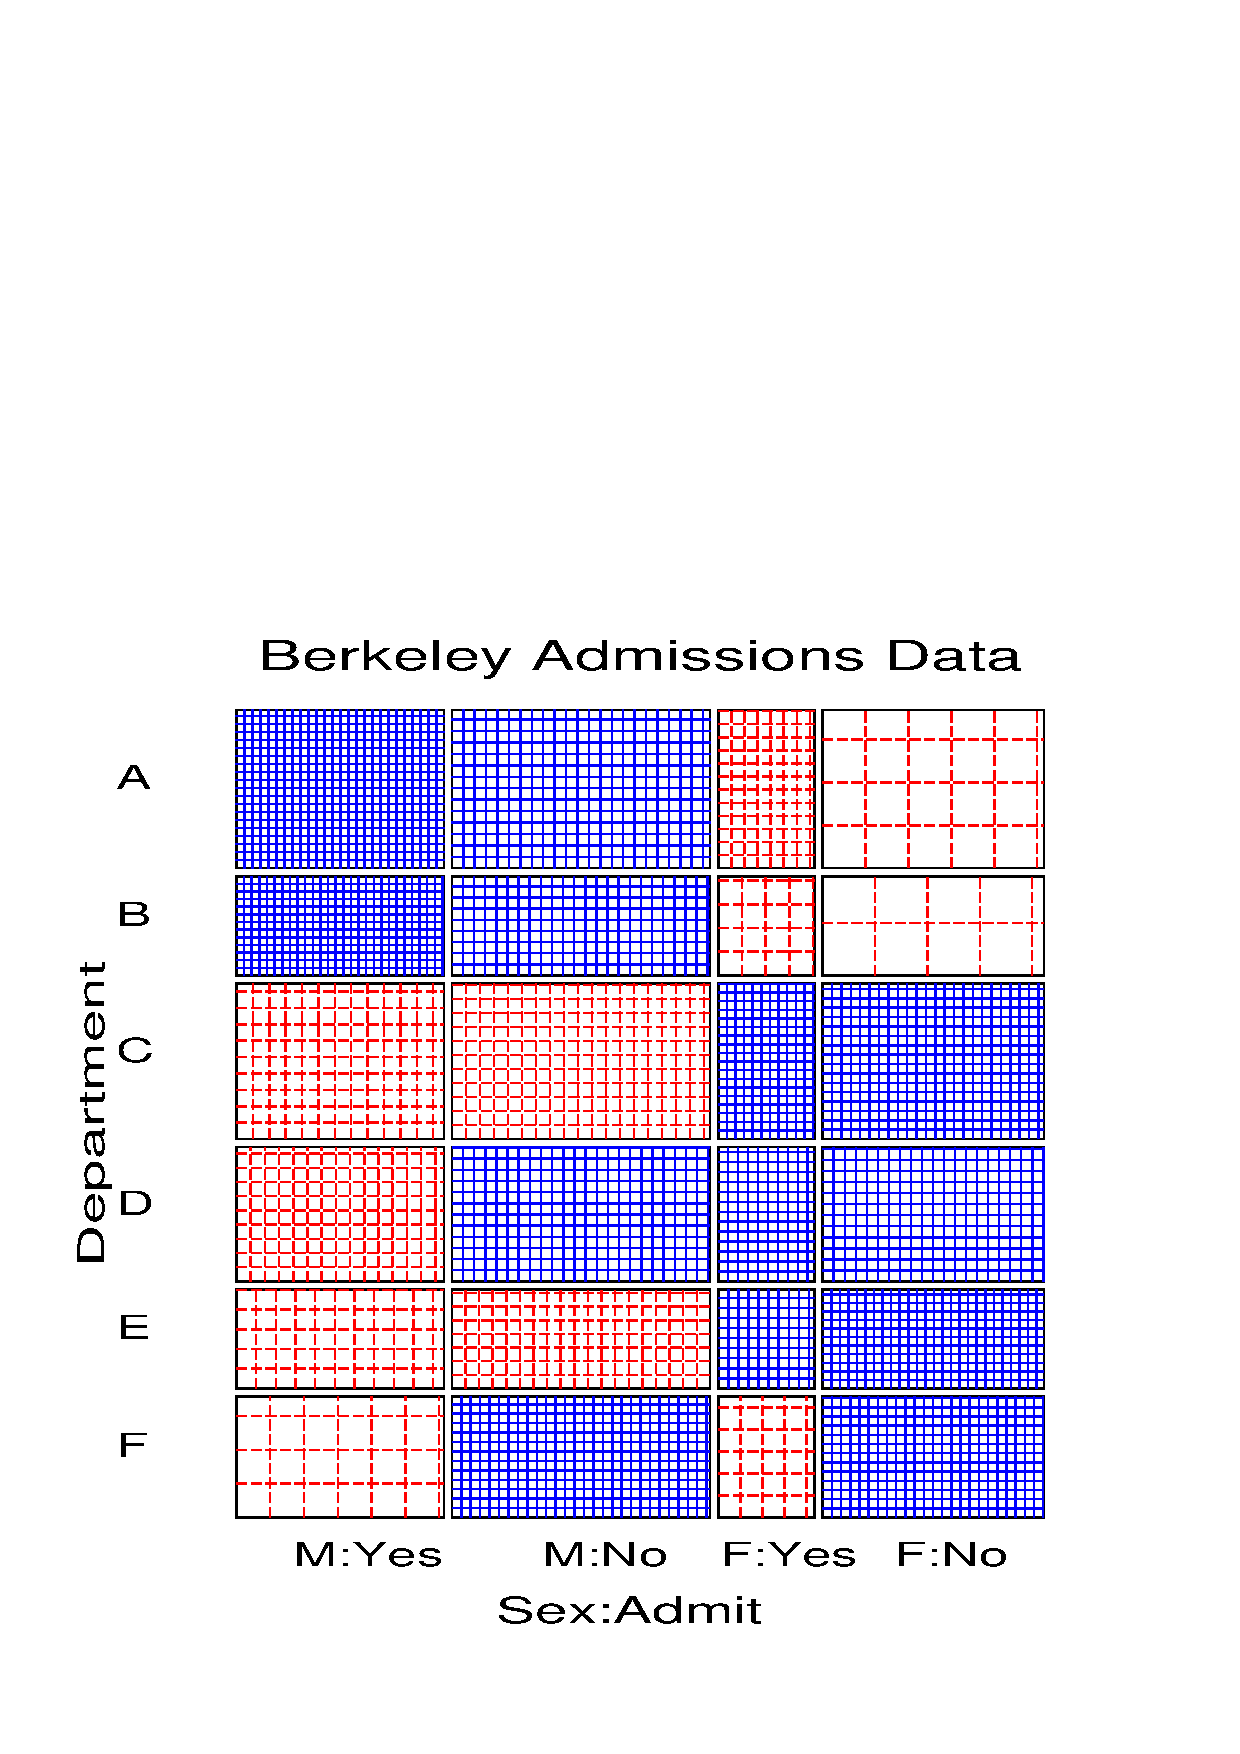
\includegraphics[scale=.5]{ch3/fig/sievebrk}
  \caption[Sieve diagram for Berkeley admissions data]{Sieve diagram for Berkeley admissions data.  The display fits a model (homogeneity) in which the combinations of sex and admission are jointly independent of department.}\label{fig:sievebrk}
\end{figure}

This sieve diagram is produced using the \texttt{sieve} module
as follows:
%% input: /users/faculty/friendly/sasuser/catdata/sievebrk.sas
%% last modified: 07-Jan-98 12:03
\begin{listing}
proc iml;
   %include sieve;
 
   vnames = \{"Department" "Sex:Admit" \};
   lnames = \{ "A" "B" "C" "D" "E" "F",
             "M:Yes" "M:No" "F:Yes"  "F:No" " " " "\};
          /*   Males       Females  */
   table = \{ 512  313      89   19,
             353  207      17    8,
             120  205     202  391,
             138  279     131  244,
              53  138      94  299,
              22  351      24  317\};
 
   font='hwpsl009';
   title  = 'Berkeley Admissions Data';
   run sieve(table, vnames, lnames, title );
quit;
\end{listing}

In this display the widths of the columns show the greater number of
male applicants than female; the greater overall admission rate for
males can be seen by comparing the ratios of widths (M:Yes / M:No) to
that of (F:Yes / F:No).
The marginal frequencies of all applicants to the various departments
are shown by the heights of the rectangles in each row.
Cells with many small squares (in blue)
correspond to those whose observed frequencies are greater than
expected under
independence.  \figref{fig:sievebrk} shows the greater numbers of
male applicants in departments A and B
(whose overall rate of admission is high) and greater numbers of female
applicants in the remaining departments (where the admission rate is low).
\end{Example}
\ixoff{sieve diagram}
